% setwd("SpecificationSims/Writeup/")
\documentclass{article}\usepackage{graphicx, color}
%% maxwidth is the original width if it is less than linewidth
%% otherwise use linewidth (to make sure the graphics do not exceed the margin)
\makeatletter
\def\maxwidth{ %
  \ifdim\Gin@nat@width>\linewidth
    \linewidth
  \else
    \Gin@nat@width
  \fi
}
\makeatother

\IfFileExists{upquote.sty}{\usepackage{upquote}}{}
\definecolor{fgcolor}{rgb}{0.2, 0.2, 0.2}
\newcommand{\hlnumber}[1]{\textcolor[rgb]{0,0,0}{#1}}%
\newcommand{\hlfunctioncall}[1]{\textcolor[rgb]{0.501960784313725,0,0.329411764705882}{\textbf{#1}}}%
\newcommand{\hlstring}[1]{\textcolor[rgb]{0.6,0.6,1}{#1}}%
\newcommand{\hlkeyword}[1]{\textcolor[rgb]{0,0,0}{\textbf{#1}}}%
\newcommand{\hlargument}[1]{\textcolor[rgb]{0.690196078431373,0.250980392156863,0.0196078431372549}{#1}}%
\newcommand{\hlcomment}[1]{\textcolor[rgb]{0.180392156862745,0.6,0.341176470588235}{#1}}%
\newcommand{\hlroxygencomment}[1]{\textcolor[rgb]{0.43921568627451,0.47843137254902,0.701960784313725}{#1}}%
\newcommand{\hlformalargs}[1]{\textcolor[rgb]{0.690196078431373,0.250980392156863,0.0196078431372549}{#1}}%
\newcommand{\hleqformalargs}[1]{\textcolor[rgb]{0.690196078431373,0.250980392156863,0.0196078431372549}{#1}}%
\newcommand{\hlassignement}[1]{\textcolor[rgb]{0,0,0}{\textbf{#1}}}%
\newcommand{\hlpackage}[1]{\textcolor[rgb]{0.588235294117647,0.709803921568627,0.145098039215686}{#1}}%
\newcommand{\hlslot}[1]{\textit{#1}}%
\newcommand{\hlsymbol}[1]{\textcolor[rgb]{0,0,0}{#1}}%
\newcommand{\hlprompt}[1]{\textcolor[rgb]{0.2,0.2,0.2}{#1}}%

\usepackage{framed}
\makeatletter
\newenvironment{kframe}{%
 \def\at@end@of@kframe{}%
 \ifinner\ifhmode%
  \def\at@end@of@kframe{\end{minipage}}%
  \begin{minipage}{\columnwidth}%
 \fi\fi%
 \def\FrameCommand##1{\hskip\@totalleftmargin \hskip-\fboxsep
 \colorbox{shadecolor}{##1}\hskip-\fboxsep
     % There is no \\@totalrightmargin, so:
     \hskip-\linewidth \hskip-\@totalleftmargin \hskip\columnwidth}%
 \MakeFramed {\advance\hsize-\width
   \@totalleftmargin\z@ \linewidth\hsize
   \@setminipage}}%
 {\par\unskip\endMakeFramed%
 \at@end@of@kframe}
\makeatother

\definecolor{shadecolor}{rgb}{.97, .97, .97}
\definecolor{messagecolor}{rgb}{0, 0, 0}
\definecolor{warningcolor}{rgb}{1, 0, 1}
\definecolor{errorcolor}{rgb}{1, 0, 0}
\newenvironment{knitrout}{}{} % an empty environment to be redefined in TeX

\usepackage{alltt}
\usepackage[height = 9in, top = 1in, width = 6.3 in]{geometry}
\usepackage{verbatim, amsmath, amsthm, amssymb}
% Palatino for rm and math | Helvetica for ss | Courier for tt
\usepackage{mathpazo} % math & rm
\linespread{1.05}        % Palatino needs more leading (space between lines)
\usepackage[scaled]{helvet} % ss
%\usepackage{courier} % tt
\normalfont
\usepackage[T1]{fontenc}

\title{A Monte Carlo Investigation of Locally Weighted Regression}
\author{Aaron Swoboda and Sam Carruthers}
\begin{document}

\maketitle




\section{Research Overview}

What do we want to know about LWR? The goal of this work is to address the following questions:
\begin{itemize}
  \item If there is no spatial relationship, will LWR default back to global OLS?
  \item Are there systematic differences in the bandwidth size selected by different techniques? How do LOOCV, Standardaized CV, Generalize CV, and the AICc compare?
  \item Which CV strategy tends to result in the most accurate coefficient estimates?
  \item What sort of spatial variation in the coefficients is necessary relative to the error to need LWR?
  \item What happens when the LWR model is misspecified?
\end{itemize}

\section{Simulation Overview}


This article simulates data under known conditions and examines the results of Locally Weighted Regression to better understand the accuracy and reliability of the technique. To do this we replicated simulations under multiple parameter combinations and ran some simulations, varying the sample size of the data set, the standard deviation of the error term in the model and the degree of spatial variation in the model coefficients. 

Each simulation was conducted as follows:
\begin{enumerate}
\item Determine the number of simulation replications and a set of values for each of the four simulation parameters: 
    \begin{enumerate}
    \item sample size
    \item variance in model error term
    \item degree of spatial variation in $\beta _1$
    \item degree of spatial variation in $\beta _2$
    \end{enumerate}
\item Select a value for each parameter from the set of values.
\item Generate the data according to the chosen parameters. 
\item Select a bandwidth for the Locally Weighted Regression (the number of observations to receive positive weights in the regression equation) from the set of all acceptable bandwidths (ranging from 5 to the sample size).
\item Estimate a Locally Weighted Regression model using the selected bandwidth for each observation in the dataset.
\item Calculate a number of metrics for the given bandwidth (cross validation scores, pseudo $R^2$, Root Mean Squared Errors, etc.).
\item Return to Step 4 and choose another bandwidth
\item Repeat Steps 4) - 7) until all bandwidths have been implemented.
\item Replicate the simulations in Steps 3) - 8) until the desired number of replications has been reached.
\item Repeat Steps 2) - 9) until all combinations of simulation parameter values have been achieved.
\end{enumerate}

We chose the following sets of simulation parameter values and replicated each simulation 100 times (for a total of $2.4\times 10^{4}$ different simulated data sets and simulations.\footnote{100 replications, 5 different sample sizes, 3 different error term variances, and 4 different degrees of spatial variation for both $\beta _1$ and $\beta _2$.}):
\begin{itemize}
\item sample size $\{$50, 200, 500, 1000$\}$
\item variance of the error term $\{2^2$, $4^2$, $6^2\}$
\item degree of spatial variation in $\beta _1$  $\{0$, .1, .2, .3$\}$
\item degree of spatial variation in $\beta _2$  $\{$0, .1, .2, .3$\}$
\end{itemize}

We kept track of the following model performance metrics, the pseudo $R^2$ of the model results, the correlation between the $\hat{\beta}$ and the true $\beta$, the percent of the observations for which we can reject the null hypothesis that $\hat{\beta}=\beta$, cross validation scores (leave one out, generalized, and standardized according to Paez), lastly the AIC score.

\subsection{Data Generation Process}

The Data Generation Process (DGP) is a modified version of a two variable linear DGP. In particular, rather than,
\begin{equation}
Y = \beta _0 + \beta _1 X_1 + \beta _2 X_2 + error,
\end{equation}
where $\beta _0$, $\beta _1$, and $\beta _2$ are constants, and $error \sim n(0, \sigma ^2)$, we construct a dataset according to Equation \eqref{eq:DGP}.
\begin{equation}\label{eq:DGP}
Y = \beta _0 + \beta _1(location) X_1 + \beta _2(location) X_2 + error
\end{equation}
The difference is that $\beta _1$ and $\beta _2$ are a function of location rather than constant. Each observation is located within a geographic coordinate system $(east, north)$ where both $east$ and $north$ values are $\sim u(0, 10)$. The functions determining $\beta _1$ and $\beta _2$ are :
\begin{eqnarray}
\beta _1 (east, north) &=& 1 + Bsv_1 * north - 5*Bsv_1 \\
\beta _2 (east, north) &=& 1 + Bsv_2 * east - 5*Bsv_2
\end{eqnarray}
The above equations show that when $Bsv_i$ is 0, the $\beta$s used to generate the dependent variable are constant across space. However, non-zero values of $Bsv_i$ imply that the marginal impact of the independent variables will differ over space. The $\beta$s used in our simulations are visualized in Figure \ref{fig:SpatVarBeta}.



\begin{figure}\label{fig:SpatVarBeta}
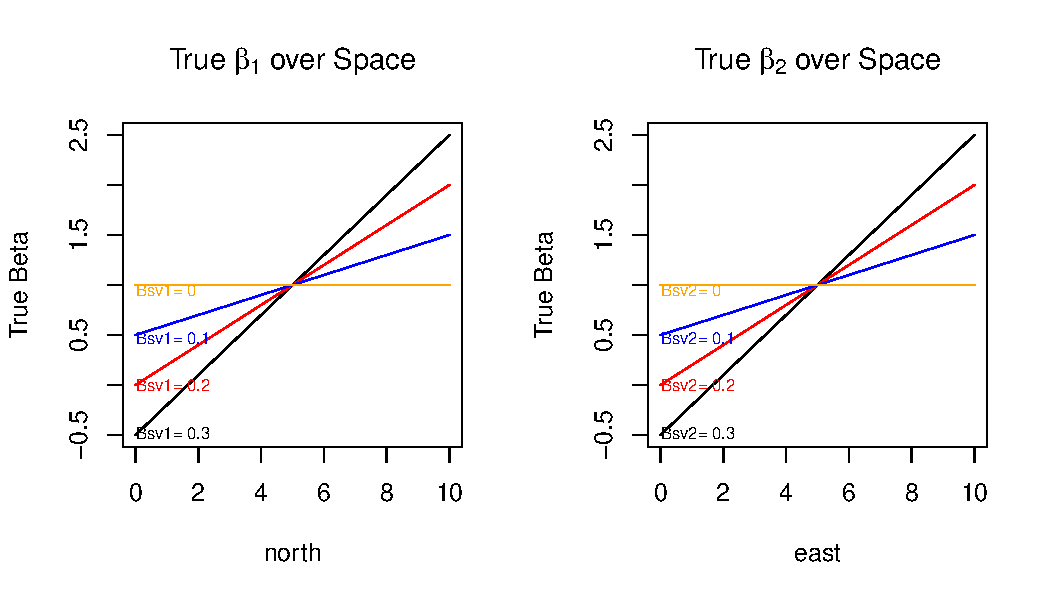
\includegraphics[width = \textwidth]{figure/SpatVarBeta.pdf}
\caption{The above images depict the different degrees of spatial variation in our DGP coefficients. Horizontal lines indicate that the coefficient is constant over space, while the steeper sloping lines indicate DGPs with higher degrees of spatial variation.}
\end{figure}
Given the different combinations of coefficient spatial variation parameters, we have data generation processes in which:
\begin{enumerate}
\item neither coefficient varies over space ($Bsv_1 = 0$ \& $Bsv_2 = 0$)
\item both coefficients vary over space ($Bsv_1 \neq 0$ \& $Bsv_2 \neq 0$)
\item only one coefficient varies over space ($Bsv_1 = 0$ \& $Bsv_2 \neq 0$ OR $Bsv_1 \neq 0$ \& $Bsv_2 = 0$)
\end{enumerate}

One of the goals of our research is to better understand the results of Locally Weighted Regression in the presence of these various underlying DGPs. 


\section{Locally Weighted Regression Description}

After generating the data, we implemented Locally Weighted Regression with the data and calculated numerous diagnostics in order to measure the performance of the regression technique and answer our research questions.

Locally Weighted Regression (LWR) is an estimation strategy allowing non-stationary model parameters. Specifically, a vector of regression parameters is estimated using Equation~\eqref{eq:LWR} for \emph{each location within the dataset,} 
\begin{equation}\label{eq:LWR}
\hat{\beta}_{location_i} =(X^TW_{location_i}X)^{-1}X^TW_{location_i}Y,
\end{equation}
where $X$ is the standard $n$ x $m$ data matrix, $Y$ the $n$ x $1$ vector of dependent variable values, and $W_{location_i}$ is an $n$ x $n$ weights matrix. We construct the weights matrix for a given $location_i$ to give positive weights to the $k$-nearest data points to $location_i$, with weights $\in [0, 1]$ and inversely related to distance between data observations and $location_i$.  Specifically, we create the weights matrix \emph{for $location_i$} with zeros on the off-diagonal and calculate the $jj$th diagonal element as,
\begin{equation}\label{eq:bisquare}
w_{jj}= 
\begin{cases} \left[1-\left(\frac{d_{ij}}{d_{ik}}\right)^2\right]^2 & \text{if $d_{ij}\leq d_{ik}$} \\
0 &\text{if $d_{ij} > d_{ik}$}
\end{cases}
\end{equation}
where $d_{ij}$ is the distance between observations $j$ and $location_i$, and $d_{ik}$ is the distance to the $k$th nearest observation to observation $i$. Thus, one of the additional parameters necessary for the implementation of LWR is selecting $k$, the local regression bandwidth. 

Theory does not provide guidance as to how many observations should receive positive weights in the local regression and must be determined by the researcher for the problem at hand. Typically, the $k$ parameter is determined by implementing LWr with several different bandwidths and then selecting the $k$ value that minimizes a model performance metric (usally a cross-validation score). This research aims to systematically compare the performance of four different cross-validation metrics used in LWR research under different, but known, data generation processes. Does choosing the LWR bandwidth through these four strategies yield similar results? If there are differences, are there patterns in how they are different?

\subsection{Bandwidth Selection Metrics}
We compare the performance of four different bandwidth selection metrics. In particular, we examine:
\begin{enumerate}
\item Leave-One-Out Cross-Validation
\item Generalized Cross-Validation 
\item Standardized Cross-Validation
\item Akaike Information Criterion
\end{enumerate}

\subsubsection{Leave-One Out Cross-Validation}

\begin{equation}
\sum (y - \hat{y}_{-i})^2
\end{equation}

\subsubsection{Generalized Cross-Validation Score}
\begin{equation}\label{eq:GCV}
  n*\sum_{i=1}^{n}\frac{(y_i-\hat{y}_i)^2}{(n-v_1)^2}, 
  \end{equation}
where $y_i$ is the dependent variable value, $\hat{y}_i$ is the predicted dependent variable value for observation $i$, and $v_1$ is the ``effective number of model parameters.''\footnote{
  $v_1=$tr(\textbf{S}), where the matrix \textbf{S} is the ``hat matrix'' which maps $y$ onto $\hat{y}$,
\begin{equation*}
  \hat{y}=\textbf{S}y,
  \end{equation*}
  and each row of \textbf{S}, $r_i$ is given by:
  \begin{equation*}
    r_i=X_i(X^TW(location_i)X)^{-1}X^TW(location_i).
    \end{equation*}
}
In an LWR model, the number of parameters to be estimated is no longer equal to the number of variables included because we allow the regression coefficients to vary over space. The GCV score calculates the ``effective'' number of model parameters, $v_1$, and penalizes the model for increasing the number of parameters without sufficient reduction in model accuracy. Taking the square root of Equation~\eqref{eq:GCV} and rearranging yields,
\begin{equation}
  \sqrt{GCV}=\sqrt{\frac{n}{n-v_1}} \sqrt{\frac{\textrm{Sum of Squared Residuals}}{n-v_1}},
\end{equation}
which approaches $\hat{\sigma}$ as $v_1$ approaches $m$ for large $n$. Henceforth, throughout the paper we report the square root of \eqref{eq:GCV} because of its similarity to $\hat{\sigma}$.  

\subsubsection{Row Standardized Cross-Validation}

Something about Paez, who wanted a CV score that was more robust to outliers.

\begin{equation}\label{eq:SCV}
\frac{\sum (y - y_{-i})^2} {\sum y}
\end{equation}

\subsubsection{Akaike Information Criterion}

\begin{equation}\label{eq:AIC}
  2*n*ln(\hat{\sigma}) + n*ln(2*\pi) + 
    n*\frac{n + v_1}{n - 2 - v_1}
    \end{equation}


\section{Which Bandwidths Do Selection Metrics Suggest?}
In this section we report on the simulation results. Specifically, we present data on the bandwidths selected by the different metrics under the different simulation conditions. The Cross Validation (CV), Generalized Cross Validation (GCV), and Akaike Information Criterion (AICc) metrics suggest strikingly similar bandwidths, while the Standardized Cross Validation metric sometimes chooses different bandwidths.

\subsection{Overall}

Table \ref{tab:bandwidthsumstats} displays the basic summary statistics of the bandwidths selected by the four different metrics across all of our simulations. Comparing the bandwidths at this level of aggregation is of limited use because we expect the selected bandwidth to vary based on the simulation conditions. For instance, the bandwidth is constrained to be smaller than the sample size of the dataset, and we expect the bandwidth selected to be a function of the degree of spatial variation in the underlying data generation process. However, the table begins to show some interesting results.


% latex table generated in R 2.15.1 by xtable 1.7-0 package
% Wed Oct 31 19:55:17 2012
\begin{table}[ht]
\begin{center}
\begin{tabular}{rrrrrrrr}
  \hline
 & min & Q1 & median & mean & Q3 & max & sd \\ 
  \hline
CV & 10 & 40 & 70 & 112 & 135 & 999 & 134 \\ 
  GCV & 5 & 40 & 70 & 111 & 135 & 999 & 134 \\ 
  SCV & 10 & 45 & 90 & 162 & 235 & 955 & 149 \\ 
  AICc & 15 & 45 & 80 & 121 & 145 & 999 & 134 \\ 
   \hline
\end{tabular}
\caption{Summary statistics for the bandwidths selected by each metric in our simulations.}
\label{tab:bandwidthsumstats}
\end{center}
\end{table}




\subsection{Bandwidth Distribution by Simulation Sample Size}

Table \ref{tab:bandwidthsbySS} breaks down the results from Table \ref{tab:bandwidthsumstats} by simulation sample size. The differences between the bandwidths selected by the Standardized Cross-Validation (SCV) metric and the other three become starker with the larger sample sizes. In general, the bandwidths selected via SCV tend to be more tightly clustered than the other three metrics. The SCV metric has the smallest standard deviation of selected bandwidths across all sample sizes. F-tests allow us to reject the null hypothesis that the variances of the selected bandwidths are equal between the SCV metric and the AICc metric (the metric with the second smallest standard deviation) for all sample sizes but 50.\footnote{$P(F_{99, 99}>\frac{22^2}{13^2}=2.86) < .001$} 

\begin{knitrout}
\definecolor{shadecolor}{rgb}{0.969, 0.969, 0.969}\color{fgcolor}\begin{kframe}
\begin{verbatim}
## [1] "Sample Size = 50"
##      min Q1 median mean Q3 max sd
## CV    10 20     30   31 40  49 12
## GCV    5 20     30   30 40  49 12
## SCV   10 25     30   29 35  49  8
## AICc  15 30     35   37 45  49  9
## [1] "Sample Size = 100"
##      min Q1 median mean Q3 max sd
## CV    10 30     45   50 65  99 24
## GCV    5 30     45   49 65  99 24
## SCV   15 45     50   51 60  99 13
## AICc  20 40     55   58 71  99 22
## [1] "Sample Size = 200"
##      min Q1 median mean  Q3 max sd
## CV    20 50     70   81 100 199 46
## GCV   15 45     70   80 100 199 46
## SCV   40 80     90   93 105 199 21
## AICc  30 55     80   90 110 199 44
## [1] "Sample Size = 500"
##      min  Q1 median mean  Q3 max  sd
## CV    30  85    120  151 170 499 107
## GCV   35  85    120  151 170 499 107
## SCV  100 190    215  217 235 480  38
## AICc  45  95    130  161 180 499 105
## [1] "Sample Size = 1000"
##      min  Q1 median mean  Q3 max  sd
## CV    55 130    185  246 260 999 210
## GCV   45 130    185  246 260 999 210
## SCV  255 380    420  421 455 955  62
## AICc  65 140    195  257 270 999 209
\end{verbatim}
\end{kframe}
\end{knitrout}




\begin{figure}\label{fig:beanplots}
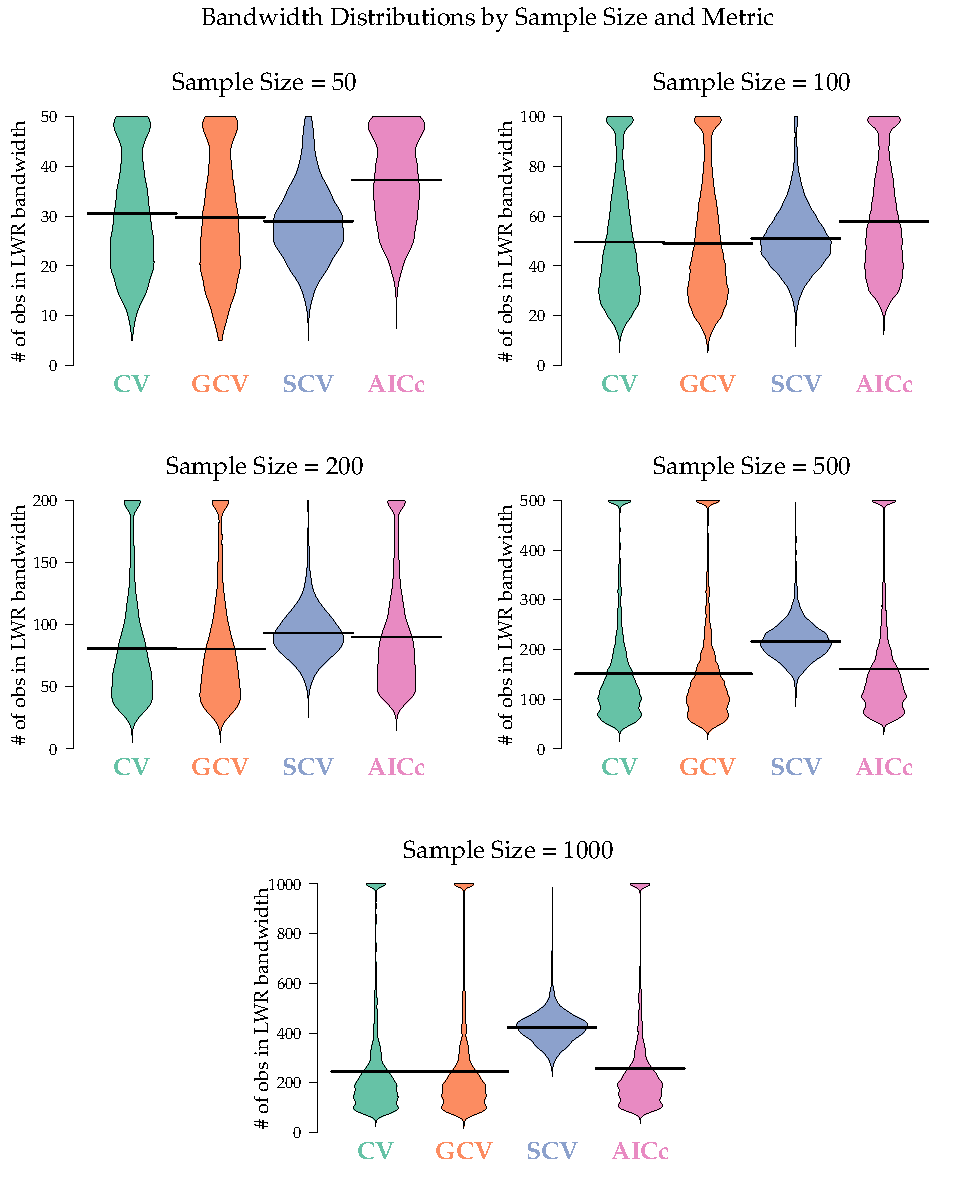
\includegraphics{figure/beanplots.pdf}
\caption{The ``beanplots'' above show the distribution of bandwidths chosen by each of the four metrics across all simulation sample sizes. Wider areas in the graph represent more data. Note that the data for the Standardized Cross Validation metric (SCV) tend to be more tightly clustered than the others. The horizontal black lines show the mean bandwidth for the given metric.}
\end{figure}

Figure \ref{fig:beanplots} visually presents the bandwidths selected by the different metrics and sample sizes of the simulations. Notice that the distributions of selected bandwidths are similar for the CV, GCV, and AICc metrics, while the SCV metric distribution stands out, especially at higher bandwidths. Additionally, note that most distributions have a cluster of selected bandwidths near the sample size. Given that one simulation parameterization included no spatial variation within the data generation coefficients, it is promising to see a cluster of large bandwidths (the more data that are considered to be ``local,'' the closer the model is to Ordinary Least Squares regression). 

\subsection{Bandwidths by Degree of Coefficient Variation}

We now proceed to examine the distributions of bandwidths by degree of spatial variation in the model coefficients. That is, let's take a single image from Figure~\ref{fig:beanplots} (Sample Size = 50) and decompose it into the 16 different plots representing the different combinations of spatial variation in the DGP coefficients (4 different levels of spatial variation for both $\beta _1$ and $\beta _2 = 16$ combinations).

Figures~\ref{fig:bandwidthsSS50bySpatVar} and \ref{fig:bandwidthsSS1000bySpatVar} display these results for sample sizes of 50 and 1000. The images are striking. The images are arranged with results of simulations containing no spatial variation in DGP coefficients in the upper left part of the page and simulations containing the most spatial variation in both DGP coefficients in the lower right part of the page. For both the small sample size (50) and the large sample size (1000), the largest possible bandwidth tends to be selected when there is no spatial variation in the DGP coefficients. As spatail variation in the DGP coefficients increases (moving down or to the right, or both), all metrics tend to select smaller bandwidths. The changes in bandwith size is most dramatic for the simulations with sample size of 1000 observations. Whereas the decrease in average bandwidth size is smooth as we moved from the upper-left to the lower-right in Figure~\ref{fig:bandwidthsSS50bySpatVar}, the average bandwidth decreases substantially as soon as we introduce \emph{any} spatial variation in the DGP coefficients in Figure~\ref{fig:bandwidthsSS1000bySpatVar}.




\begin{figure}\label{fig:bandwidthsSS50bySpatVar}
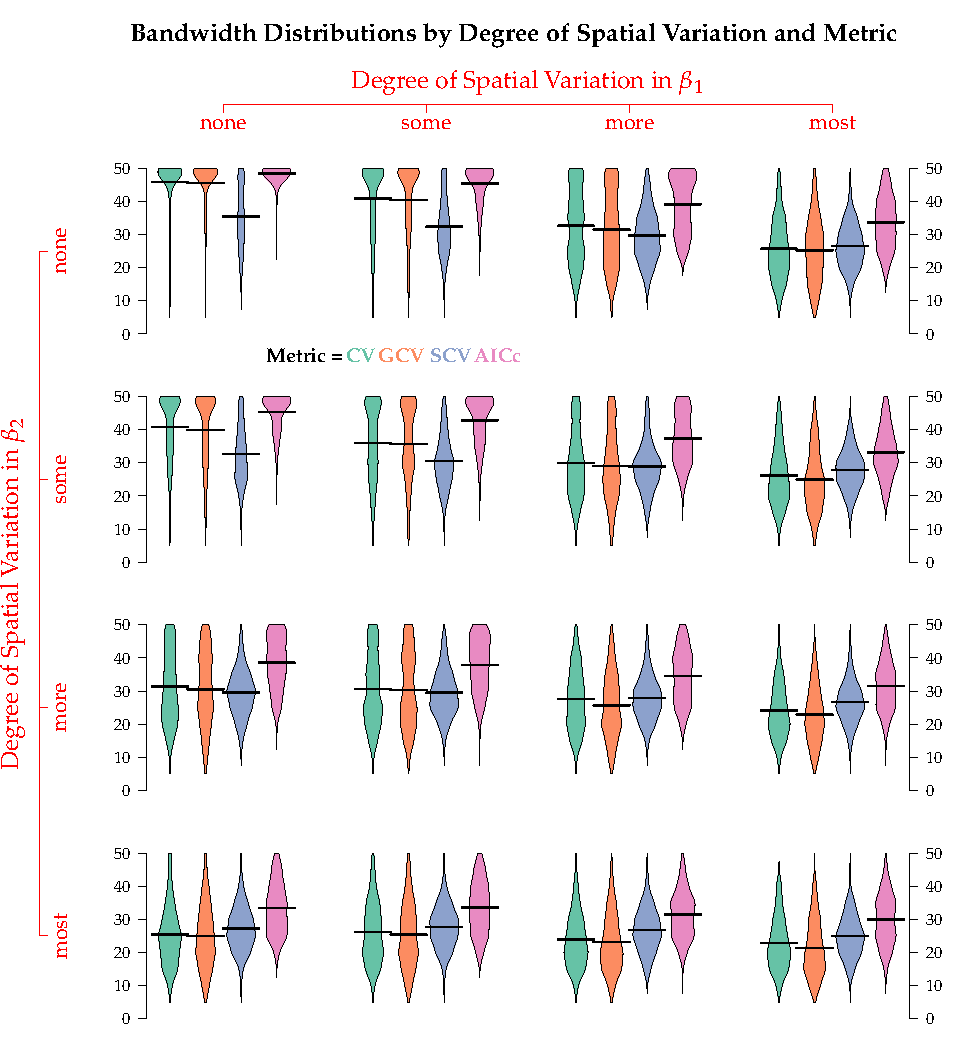
\includegraphics{figure/bandwidthsSS50bySpatVar.pdf}
\caption{These images display ``beanplots'' of the bandwidths selected by each metric for each combination of $\beta _1$ and $\beta _2$ spatial variation for a sample size of 50 data points. Note how the distributions change from the upper left (no spatial variation in either coeffient) to the lower right (the most spatial variation in both coefficients). The size of the selected bandwidth tends to be inversely related to the degree of spatial variation in the coefficients.}
\end{figure}




\begin{figure}\label{fig:bandwidthsSS1000bySpatVar}
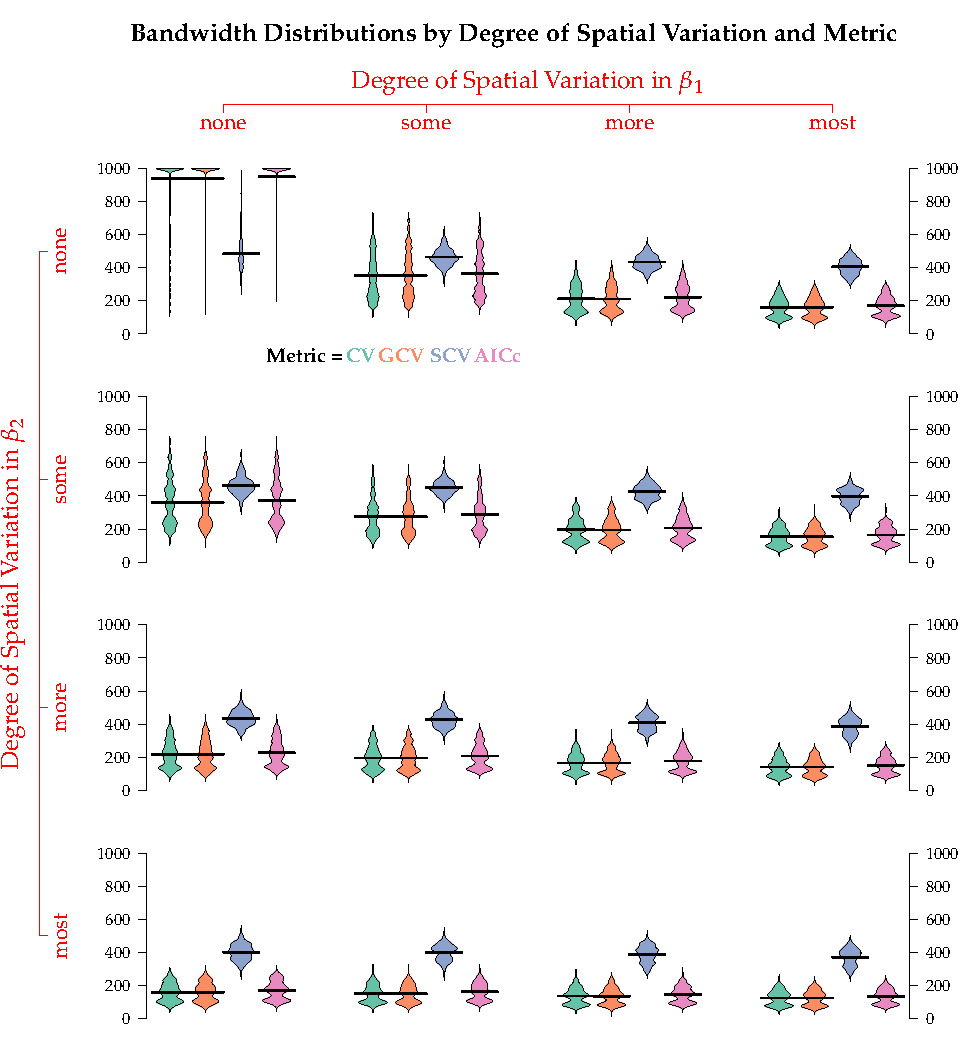
\includegraphics{figure/bandwidthsSS1000bySpatVar.pdf}
\caption{These images display ``beanplots'' of the bandwidths selected by each metric for each combination of $\beta _1$ and $\beta _2$ spatial variation for a sample size of 1000 data points. Note how the distributions change from the upper left (no spatial variation in either coeffient) to the lower right (the most spatial variation in both coefficients). The size of the selected bandwidth tends to be inversely related to the degree of spatial variation in the coefficients.}
\end{figure}

\subsection{Bandwidth and Error Term Variances}

None of the previous analysis has examined the role of the Data Generation Process error term variance. We ran each simulation combination of sample size, degree of spatial variation in $\beta _1$ and degree of spatial variation in $\beta _2$ with three different DGP error term variances, $\sigma ^2 \in \{2^2, 4^2, 6^2\}$. This section describes the bandwidths selected by the four different selection metrics across these differing DGPs. Larger error term variances serve to ``hide'' the underlying model in noise. We therefore hypothesize that, all other things equal, larger error term variances will lead to higher bandwidths selected, as the Locally Weighted Regression will have a more difficult time ``finding'' spatial variation in the regression coefficients, and it will therefore select a larger bandwidth.

Figures~\ref{fig:bandwidthsSS50bySpatVarError} and \ref{fig:bandwidthsSS1000bySpatVarError} are similar to Figures~\ref{fig:bandwidthsSS50bySpatVar} and \ref{fig:bandwidthsSS1000bySpatVar}, with a few important differences. First, rather than plotting the entire bandwidth distribution density for a given simulation scenario, we make a line plot showing the middle 90 percent of the distribution and denote the mean selected bandwidth. This decision helps to fit the large amount of data into Figures~\ref{fig:bandwidthsSS50bySpatVarError} and \ref{fig:bandwidthsSS1000bySpatVarError}.




\begin{figure}\label{fig:bandwidthsSS50bySpatVarError}
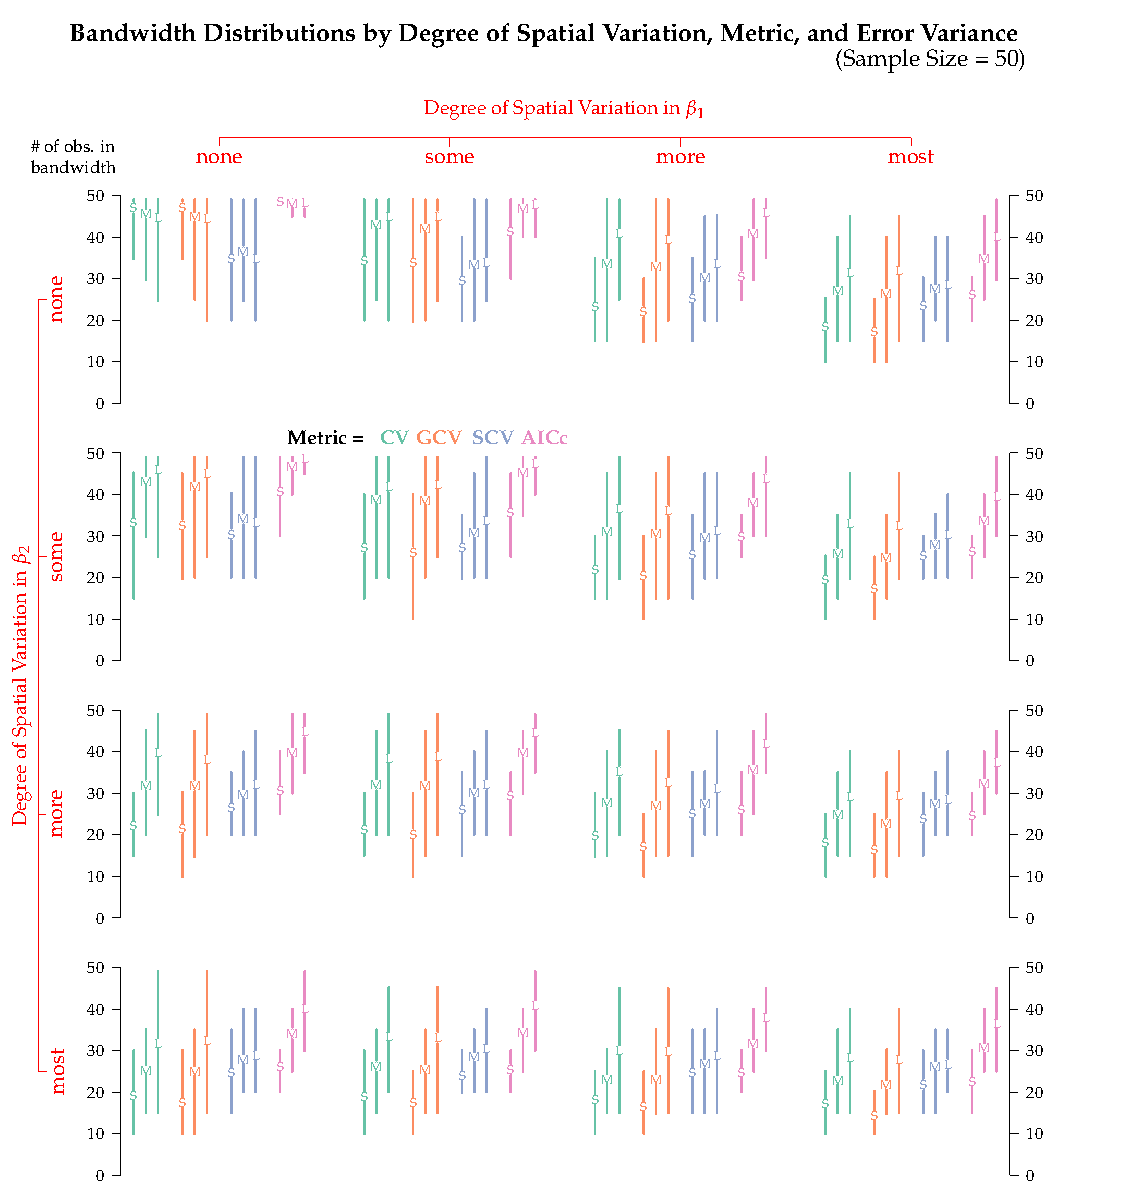
\includegraphics{figure/bandwidthsSS50bySpatVarError.pdf}
\caption{These images display the bandwidths selected by each metric for each combination of $\beta _1$ and $\beta _2$ spatial variation and DGP error variance for a sample size of 50 data points. Note how the distributions change from the upper left (no spatial variation in either coeffient) to the lower right (the most spatial variation in both coefficients). The size of the selected bandwidth tends to be inversely related to the degree of spatial variation in the coefficients.}
\end{figure}



\section{How Accurate are the LWR Coefficient Estimates?}

Rather than just looking at the bandwidths selected, researchers are probably more interested in the accuracy of the model predictions, specifically with regard to the model coefficients. In particular, does LWR tend to overfit the data by choosing small bandwidths and spurious coefficients? In this section we compare the estimated model coefficients to the true model coefficients to better understand the reliability of the LWR procedure.


\section{What Happens When the Model is Misspecified?}

In previous sections we assumed that the model to be estimated using LWR was properly specified. That is, bothe variables ($X_1$ and $X_2$) are included and their coefficients are allowed to vary over space to reflect the true data generation process. This section relaxes the assumption of a perfectly specified model and omits one variable in the regression. Our new regression equation becomes:
\begin{equation}
y = \alpha (location) + \beta _1 (location) X_1 + error
\end{equation}

An important question to consider in these circumstances is, ``What happens when the omitted variable had a spatially varying coefficient, but the included variable coefficients are stationary?'' Does LWR choose a large bandwidth and reflect the stationarity of the included model parameters? Does LWR select a small bandwidth and estimate spatially varying intercept terms? If so, what are the impacts on our estimates of the stationary parameter?


\section{Simulation Code}
This section includes the code used to run our simulations.

The Data Generation Process is achieved using the \texttt{DataGen} function, the code for which is given below. 
\begin{knitrout}
\definecolor{shadecolor}{rgb}{0.969, 0.969, 0.969}\color{fgcolor}\begin{kframe}
\begin{alltt}
\hlfunctioncall{source}(\hlstring{"../SimFunctions.R"})
DataGen
\end{alltt}
\begin{verbatim}
## function (sample.size, error.sd, B1.spatial.var, B2.spatial.var) 
## {
##     n = sample.size
##     east = runif(sample.size) * 10
##     north = runif(sample.size) * 10
##     indep.var1 = runif(sample.size) * 10
##     indep.var2 = runif(sample.size) * 10
##     trueB0 = 0
##     trueB1 = B1.spatial.var * north + 1 - 5 * B1.spatial.var
##     trueB2 = B2.spatial.var * east + 1 - 5 * B2.spatial.var
##     error = rnorm(sample.size, 0, error.sd)
##     dep.var = trueB0 + indep.var1 * trueB1 + indep.var2 * trueB2 + 
##         error
##     output = data.frame(dep.var, north, east, indep.var1, indep.var2, 
##         trueB0, trueB1, trueB2, error)
##     output
## }
\end{verbatim}
\end{kframe}
\end{knitrout}


The simulations were run and initial metrics calculated in a recent run of \texttt{uberScript.R}. It contains the following code:

\begin{knitrout}
\definecolor{shadecolor}{rgb}{0.969, 0.969, 0.969}\color{fgcolor}\begin{kframe}
\begin{alltt}
\hlcomment{# set our simulation parameters}
Replications = 100
sample.size = \hlfunctioncall{c}(50, 100, 200, 500, 1000)
error.sd = \hlfunctioncall{c}(2, 4, 6)
B1.spatial.var = \hlfunctioncall{c}(0, .1, .2, .3)
B2.spatial.var = \hlfunctioncall{c}(0, .1, .2, .3)
\hlcomment{# now march through the different parameter combinations running the simulations}
\hlfunctioncall{for}( i in 1:meta.sim.num) \{ 
  start = \hlfunctioncall{Sys.time}()
  simRepOut = \hlfunctioncall{simulationReplicator}(Replications, sim.parameters[i, ], MC = TRUE)
  simOut = \hlfunctioncall{simRepReorganizer}(simRepOut)
  
  R2Output[\hlfunctioncall{as.character}(sim.parameters[i, \hlstring{"sample.size"}]),
           \hlfunctioncall{as.character}(sim.parameters[i, \hlstring{"error.sd"}]),
           \hlfunctioncall{as.character}(sim.parameters[i, \hlstring{"B1.spatial.var"}]),
           \hlfunctioncall{as.character}(sim.parameters[i, \hlstring{"B2.spatial.var"}]), , ] = simOut[[1]]
  
  MetricOutput[\hlfunctioncall{as.character}(sim.parameters[i, \hlstring{"sample.size"}]),
               \hlfunctioncall{as.character}(sim.parameters[i, \hlstring{"error.sd"}]),
               \hlfunctioncall{as.character}(sim.parameters[i, \hlstring{"B1.spatial.var"}]),
               \hlfunctioncall{as.character}(sim.parameters[i, \hlstring{"B2.spatial.var"}]), , , ] = simOut[[2]]
  end = \hlfunctioncall{Sys.time}()
  \hlfunctioncall{print}(\hlfunctioncall{paste}(\hlstring{"For loop"}, i,\hlstring{"of"}, meta.sim.num))
  \hlfunctioncall{print}(\hlfunctioncall{round}(\hlfunctioncall{difftime}(end, start, units = \hlstring{"m"}), 2))
  \hlfunctioncall{save}(R2Output, MetricOutput, file = \hlstring{"SpecificationSims/uberScriptOutput.RData"})
\}
\end{alltt}
\end{kframe}
\end{knitrout}


I'm not going to run that code here (it took almost a month to run on the R Server), but let's load up the results and start to look at them. Or at least come up with some questions to ask of the data and a plan for the future.

\begin{knitrout}
\definecolor{shadecolor}{rgb}{0.969, 0.969, 0.969}\color{fgcolor}\begin{kframe}
\begin{alltt}
\hlfunctioncall{load}(\hlstring{"../Data/uberScriptOutput20120919.RData"})
\hlfunctioncall{dimnames}(MetricOutput)
\end{alltt}
\begin{verbatim}
## $ss
## [1] "50"   "100"  "200"  "500"  "1000"
## 
## $error.sd
## [1] "2" "4" "6"
## 
## $B1sv
## [1] "0"   "0.1" "0.2" "0.3"
## 
## $B2sv
## [1] "0"   "0.1" "0.2" "0.3"
## 
## $simNum
##   [1] "1"   "2"   "3"   "4"   "5"   "6"   "7"   "8"   "9"   "10"  "11"  "12"  "13" 
##  [14] "14"  "15"  "16"  "17"  "18"  "19"  "20"  "21"  "22"  "23"  "24"  "25"  "26" 
##  [27] "27"  "28"  "29"  "30"  "31"  "32"  "33"  "34"  "35"  "36"  "37"  "38"  "39" 
##  [40] "40"  "41"  "42"  "43"  "44"  "45"  "46"  "47"  "48"  "49"  "50"  "51"  "52" 
##  [53] "53"  "54"  "55"  "56"  "57"  "58"  "59"  "60"  "61"  "62"  "63"  "64"  "65" 
##  [66] "66"  "67"  "68"  "69"  "70"  "71"  "72"  "73"  "74"  "75"  "76"  "77"  "78" 
##  [79] "79"  "80"  "81"  "82"  "83"  "84"  "85"  "86"  "87"  "88"  "89"  "90"  "91" 
##  [92] "92"  "93"  "94"  "95"  "96"  "97"  "98"  "99"  "100"
## 
## $optimized
##  [1] "AICc"     "corB0"    "corB1"    "corB2"    "CV"       "GCV"      "R2"      
##  [8] "RMSE.B0"  "RMSE.B1"  "RMSE.B2"  "SCV"      "ttest%B0" "ttest%B1" "ttest%B2"
## 
## $metric
##  [1] "bandwidths" "B0.cor"     "B1.cor"     "B2.cor"     "B0.RMSE"    "B1.RMSE"   
##  [7] "B2.RMSE"    "B0.t.perc"  "B1.t.perc"  "B2.t.perc"  "GCV"        "SCV"       
## [13] "CV"         "AICc"       "R2"
\end{verbatim}
\begin{alltt}
\hlfunctioncall{dimnames}(R2Output)
\end{alltt}
\begin{verbatim}
## $ss
## [1] "50"   "100"  "200"  "500"  "1000"
## 
## $error.sd
## [1] "2" "4" "6"
## 
## $B1sv
## [1] "0"   "0.1" "0.2" "0.3"
## 
## $B2sv
## [1] "0"   "0.1" "0.2" "0.3"
## 
## $simNum
##   [1] "1"   "2"   "3"   "4"   "5"   "6"   "7"   "8"   "9"   "10"  "11"  "12"  "13" 
##  [14] "14"  "15"  "16"  "17"  "18"  "19"  "20"  "21"  "22"  "23"  "24"  "25"  "26" 
##  [27] "27"  "28"  "29"  "30"  "31"  "32"  "33"  "34"  "35"  "36"  "37"  "38"  "39" 
##  [40] "40"  "41"  "42"  "43"  "44"  "45"  "46"  "47"  "48"  "49"  "50"  "51"  "52" 
##  [53] "53"  "54"  "55"  "56"  "57"  "58"  "59"  "60"  "61"  "62"  "63"  "64"  "65" 
##  [66] "66"  "67"  "68"  "69"  "70"  "71"  "72"  "73"  "74"  "75"  "76"  "77"  "78" 
##  [79] "79"  "80"  "81"  "82"  "83"  "84"  "85"  "86"  "87"  "88"  "89"  "90"  "91" 
##  [92] "92"  "93"  "94"  "95"  "96"  "97"  "98"  "99"  "100"
## 
## $R2
## [1] "OLS" "LWR"
\end{verbatim}
\end{kframe}
\end{knitrout}


\end{document}
